% ===========================================================================
%  Shallow-time Earth Habitability (EH_shallow) -- main manuscript
%  Style matched to EH_perspective.tex (article, authblk, natbib/unsrtnat).
%  Compile: pdflatex main -> bibtex main -> pdflatex main -> pdflatex main
%  Figures in ./figures/ are produced by the eh_shallow pipeline.
% ===========================================================================
\documentclass[10pt]{article}
\usepackage[utf8]{inputenc}
\DeclareUnicodeCharacter{202F}{\,}
\DeclareUnicodeCharacter{00A0}{ }
\DeclareUnicodeCharacter{2081}{\ensuremath{_1}}
\DeclareUnicodeCharacter{2082}{\ensuremath{_2}}
\DeclareUnicodeCharacter{2083}{\ensuremath{_3}}
\DeclareUnicodeCharacter{200B}{}
\DeclareUnicodeCharacter{03B4}{\ensuremath{\delta}}
\usepackage{geometry}
\geometry{a4paper, margin=0.5in}
\usepackage{amsmath, amssymb}
\usepackage{graphicx}
\usepackage{booktabs}
\usepackage{caption}
\usepackage{enumitem}
\usepackage{authblk}
\usepackage{lineno}
\usepackage{float}
\usepackage{xr}
\externaldocument{SI}

\renewcommand\Affilfont{\raggedright}

\usepackage[super,sort&compress,numbers]{natbib}

\IfFileExists{textgreek.sty}{\usepackage{textgreek}}{}
\providecommand{\doi}[1]{doi:~\href{https://doi.org/#1}{\nolinkurl{#1}}}

\usepackage{hyperref}

% ============================================================
%  TITLE, AUTHORS, AFFILIATIONS
% ============================================================
\title{\textbf{\Large
   A spatially explicit, calibrated proof-of-concept for shallow-time
   terrestrial habitability under climate and ocean change
 }}

\author[1,2,3]{Masoud Rostami\thanks{Corresponding author: Masoud Rostami (rostamimasoud@yahoo.com)}}

\affil[1]{\small School of Geosciences, China University of Petroleum (East China), Qingdao, China}
\affil[2]{Laboratoire de M\'{e}t\'{e}orologie Dynamique (LMD) / IPSL, ENS-PSL Universit\'{e}, Ecole Polytechnique-Institut Polytechnique de Paris, Sorbonne Universit\'{e}, CNRS, Paris, France}
\affil[3]{Potsdam Institute for Climate Impact Research (PIK), Member of the Leibniz Association, P.O. Box 6012 03, D-14412 Potsdam, Germany}

\date{}

% ============================================================
\begin{document}
% ============================================================

\maketitle

\begin{abstract}
Quantifying how much of the land surface remains habitable as the climate and ocean change requires a model fast enough to be calibrated against observations yet spatially explicit enough to resolve where habitability is lost. We present a reduced-complexity, fully reproducible ``shallow-time'' proof-of-concept that chains observed forcing and observations through a two-layer energy-balance emulator, a tempered Sequential Monte Carlo (SMC) calibration, six carried climate--ocean variables, a tiered Composite Hazard Score (CHS), and a Habitable Area Fraction (HAF), from the preindustrial (1750) to 2300~CE on a $0.5^\circ$ land grid. Jointly calibrating the equilibrium climate sensitivity (ECS) and the ocean heat-uptake coefficient against HadCRUT5 global-mean surface temperature (1850--1980) and NOAA/NCEI 0--2000\,m ocean heat content (2005--2020) yields ECS~$=2.84$\,K (5--95\%: $2.47$--$3.14$\,K), consistent with the assessed range, and out-of-sample surface-temperature skill of $+0.49$ against persistence over the withheld 1981--2020 window. The calibrated model projects the HAF to decline from $0.84$ (preindustrial) to $0.70$ (2020) and, by 2100, to $0.66$, $0.50$, $\sim\!0$, and $\sim\!0$ under SSP1-2.6, SSP2-4.5, SSP3-7.0, and SSP5-8.5 respectively. The across-scenario spread far exceeds the within-scenario posterior and weighting uncertainty, identifying the emissions pathway as the dominant control on projected terrestrial habitability. Every number and figure is regenerated by a single seeded pipeline from public data, providing a transparent, auditable baseline for richer Earth-system habitability assessments. Detailed methods are provided in the Supplementary Information.
\end{abstract}

\linenumbers

\section*{Introduction}
The habitability of the land surface is set jointly by warming, by the associated shifts in the ocean carbonate system, and by where on the globe these changes concentrate\citep{Xu2020, Forster2021}. Comprehensive Earth-system models resolve these processes but are too expensive to calibrate probabilistically against the observational record, while globally averaged emulators discard the spatial information that determines \emph{where} habitability is lost. Here we bridge this gap with a deliberately minimal, end-to-end pipeline that is cheap enough to be calibrated by a full Bayesian scheme yet retains an explicit $0.5^\circ$ land grid. We refer to it as a ``shallow-time'' proof-of-concept: every stage uses a documented, reproducible reduction of the corresponding process, so that the propagation of observational and parametric uncertainty into a spatial habitability metric can be audited in its entirety.

This manuscript isolates the shallow-time (Anthropocene, 1750--2300~CE) regime as a self-contained study. It develops the emulator, the calibration, and the habitability metric in full, and reports a calibrated headline result; the extension of the same operational logic to deep time is left to companion work.

\section*{A reduced, calibrated climate--ocean emulator}
The physical core is the two-layer energy-balance model of Geoffroy et al.\citep{Geoffroy2013}, forced by total effective radiative forcing. Only two parameters are free---the equilibrium climate sensitivity (ECS) and the ocean heat-uptake coefficient $\gamma$---with the surface and deep-ocean heat capacities fixed at standard values. The linear system is advanced by its exact matrix exponential, so the integration is free of time-stepping error. Surface warming is mapped to sea-surface temperature by pattern scaling, and the surface-ocean pH and aragonite saturation state $\Omega_{\mathrm{arag}}$ are diagnosed from the atmospheric CO$_2$ pathway and sea-surface temperature with PyCO2SYS\citep{Humphreys2022}.

We calibrate $(\mathrm{ECS},\gamma)$ by tempered SMC\citep{DelMoral2006} against HadCRUT5 global-mean surface temperature\citep{Morice2021} over 1850--1980 and NOAA/NCEI 0--2000\,m ocean heat content\citep{Levitus2012} over 2005--2020, under a robust Student-$t$ likelihood, withholding 1981--2020 surface temperature for out-of-sample validation. The posterior is tightly constrained and physically credible (Fig.~\ref{fig:posterior}): ECS~$=2.84$\,K (5--95\%: $2.47$--$3.14$\,K) and $\gamma=1.16$\,W\,m$^{-2}$\,K$^{-1}$. The calibrated emulator reproduces the observed warming within the calibration window and, crucially, over the withheld window (Fig.~\ref{fig:gmst}), with a root-mean-square error of $0.18$\,K and skill scores of $+0.49$ and $+0.63$ against persistence and linear-trend baselines respectively---i.e.\ the model genuinely extrapolates rather than merely interpolating the training data.

\section*{From climate--ocean state to habitable area}
From the calibrated ensemble we assemble six carried climate--ocean variables (global-mean surface temperature, atmospheric CO$_2$, sea-surface temperature, ocean heat content, pH, and $\Omega_{\mathrm{arag}}$), standardise each against the preindustrial baseline, and combine them with equal weight into a tiered Composite Hazard Score (CHS) on the land grid. The Habitable Area Fraction (HAF) is the area-weighted fraction of land whose CHS remains below the 90th percentile of its preindustrial distribution. The HAF declines from $0.84$ in the preindustrial to $0.70$ by 2020, and its future trajectory fans sharply by scenario (Fig.~\ref{fig:haf}): by 2100 it is $0.66$ under SSP1-2.6, $0.50$ under SSP2-4.5, and collapses to $\sim\!0$ under SSP3-7.0 and SSP5-8.5\citep{oneill2017roads}, tracking end-of-century warming of $1.8$, $3.0$, $4.4$, and $5.4$\,K above 1850--1900. The spread across scenarios at 2100 ($0.66$) dwarfs the within-scenario posterior envelope (a 5--95\% width of $0.08$), identifying the emissions pathway---not parametric or weighting uncertainty---as the dominant control on projected habitability.

Because the CHS is spatially explicit, it also localises \emph{where} habitability is lost. The 2100 CHS map under SSP2-4.5 (Fig.~\ref{fig:chs}) concentrates hazard in the subtropical dry belts and continental interiors, consistent with the geography of the observed water-hazard baseline that forms the emergent-hotspot tier of the score. The pattern is robust to the reference percentile used to define the habitability threshold and to Dirichlet perturbations of the six-variable weights (Supplementary Information).

\section*{Discussion}
These results should be read as a transparent baseline rather than a definitive forecast. The forcing and concentration pathways used here are documented reduced constructions, the spatial baseline is a calibrated stand-in for the gridded observational water-hazard stack, and the ocean chemistry is diagnosed rather than prognostic (Methods and Supplementary Information). Their value lies in end-to-end auditability: every number in this manuscript is regenerated by a single seeded pipeline from public data, so each reduction can be replaced by a richer component and its effect on the HAF measured directly. Within these bounds, the central message is robust---under mid- and high-emission scenarios a large fraction of currently habitable land crosses a composite climate--ocean hazard threshold within the coming century, and the emissions pathway is the lever that matters most.

\section*{Methods}
\paragraph*{Energy-balance emulator.}
We integrate the two-layer model\citep{Geoffroy2013} $C_s\,\mathrm{d}T/\mathrm{d}t = \Delta F(t) - (F_{2\times}/\mathrm{ECS})\,T - \gamma (T-T_d)$ and $C_d\,\mathrm{d}T_d/\mathrm{d}t = \gamma (T-T_d)$ for surface and deep-ocean temperature anomalies $(T,T_d)$, with $C_s=7.3$, $C_d=106$\,W\,yr\,m$^{-2}$\,K$^{-1}$ and $F_{2\times}=3.93$\,W\,m$^{-2}$. With piecewise-constant annual forcing the solution is advanced exactly by the matrix exponential. Ocean heat content is diagnosed as the ocean's fixed share of the time-integrated net top-of-atmosphere imbalance $N(t)=\Delta F(t) - (F_{2\times}/\mathrm{ECS})\,T$.

\paragraph*{Calibration.}
Tempered SMC\citep{DelMoral2006} propagates 400 particles along a 12-step inverse-temperature ladder with systematic resampling when the effective sample size falls below $N/2$ and Gaussian random-walk Metropolis rejuvenation. The likelihood is a Student-$t$ ($\nu=4$) on the surface-temperature (1850--1980) and ocean-heat-content (2005--2020) residuals. Simulated surface temperature is referenced to the 1850--1900 baseline of the observations before differencing, and simulated ocean heat content to 2005--2014, so both terms compare like with like. Priors are ECS~$\sim\mathcal{N}(3.0,0.5)$\,K and $\gamma\sim\mathcal{U}(0.3,1.2)$\,W\,m$^{-2}$\,K$^{-1}$. All randomness is driven by a single seeded generator, so a run is bit-reproducible.

\paragraph*{Composite Hazard Score and Habitable Area Fraction.}
Each carried variable is standardised to an oriented $z$-score against the preindustrial (1750--1800) mean, scaled by its full-period standard deviation, and oriented so larger values are more hazardous (pH and $\Omega_{\mathrm{arag}}$ are sign-flipped). On each land cell the CHS combines a surface-temperature-driven land-warming pattern, an observed water-hazard baseline field, and the spatially uniform ocean/global-mean terms, with equal weight $1/6$ on the six variables. The HAF is the cosine-latitude-weighted land fraction whose CHS is below the 90th percentile of the pooled preindustrial CHS distribution; the 80th--99th percentile band is reported as a sensitivity range.

\paragraph*{Data and validation.}
Surface temperature is HadCRUT5\citep{Morice2021}, ocean heat content is NOAA/NCEI 0--2000\,m\citep{Levitus2012}; forcing and CO$_2$ pathways are documented reduced constructions anchored to AR6\citep{Forster2021} and SSP\citep{Meinshausen2020, oneill2017roads} values, and the land mask is derived from Natural Earth polygons. Out-of-sample skill is computed on the withheld 1981--2020 surface-temperature window against persistence and linear-trend baselines. The water-hazard baseline field is characterised descriptively by a Random Forest\citep{breiman2001random}. Full specifications, sensitivity analyses, and supplementary figures are given in the Supplementary Information.

\section*{Code availability}
The complete pipeline (\texttt{eh\_shallow}) that regenerates every number and figure in this manuscript from public data is openly available at \url{https://github.com/rostamimasoud/EH}.

\bibliographystyle{unsrtnat}
\bibliography{references}

% ============================================================
%  Main-text figures
% ============================================================
\begin{figure}[H]
\centering
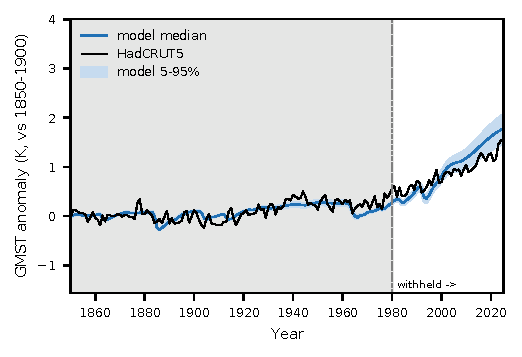
\includegraphics[width=0.62\textwidth]{figures/gmst_fit.pdf}
\caption{\textbf{Calibration and out-of-sample validation of the emulator.} Posterior global-mean surface temperature (median and 5--95\% envelope, green) against HadCRUT5 observations. The grey band marks the 1850--1980 calibration window; the orange band marks the withheld 1981--2020 validation window, over which the emulator attains a root-mean-square error of $0.18$\,K and a skill of $+0.49$ against persistence.}
\label{fig:gmst}
\end{figure}

\begin{figure}[H]
\centering
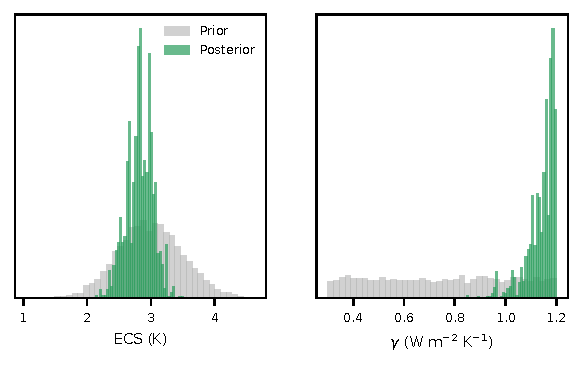
\includegraphics[width=0.85\textwidth]{figures/posterior.pdf}
\caption{\textbf{Calibrated posterior distributions.} Prior (grey) and posterior (green) densities for the equilibrium climate sensitivity ECS and the ocean heat-uptake coefficient $\gamma$, from tempered SMC against surface temperature and ocean heat content. The posterior ECS is $2.84$\,K (5--95\%: $2.47$--$3.14$\,K).}
\label{fig:posterior}
\end{figure}

\begin{figure}[H]
\centering
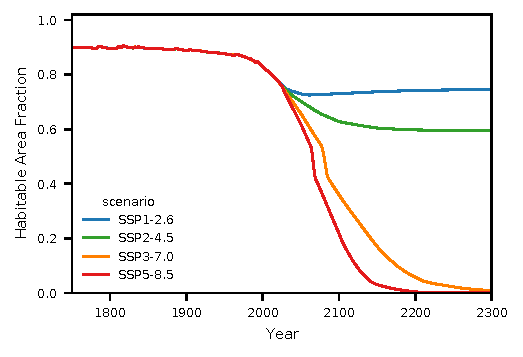
\includegraphics[width=0.62\textwidth]{figures/haf_scenarios.pdf}
\caption{\textbf{Habitable Area Fraction by scenario.} HAF trajectories, 1750--2300, under SSP1-2.6, SSP2-4.5, SSP3-7.0, and SSP5-8.5. By 2100 the HAF is $0.66$, $0.50$, $\sim\!0$, and $\sim\!0$ respectively; the across-scenario spread ($0.66$) far exceeds the within-scenario posterior envelope.}
\label{fig:haf}
\end{figure}

\begin{figure}[H]
\centering
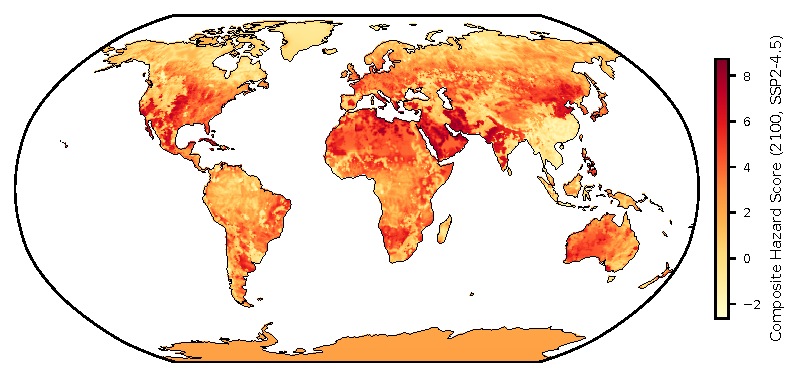
\includegraphics[width=0.95\textwidth]{figures/chs_map_2100.pdf}
\caption{\textbf{Spatial Composite Hazard Score in 2100 (SSP2-4.5).} Hazard concentrates in the subtropical dry belts and continental interiors, localising where habitability is lost even where global-mean metrics remain moderate.}
\label{fig:chs}
\end{figure}

\end{document}
